\normaltrue \difficilefalse \tdifficilefalse
\correctiontrue
%\UPSTIidClasse{11} % 11 sup, 12 spé
%\newcommand{\UPSTIidClasse}{11}

\exer{ $\star$ \label{B2:16:71}}
%% CCP MP 2007
\setcounter{question}{0}\UPSTIcompetence[2]{B2-16}
\index{Compétence B2-16}

\index{Robovolc}
\index{Hyperstatisme}

\ifcorrection
\else
\textbf{Pas de corrigé pour cet exercice.}
\fi


\question{Calculer l'hyperstatisme du modèle plan du mécanisme global de la pince (\autoref{fig_23}).}
\ifprof
Le graphe de liaisons est donné figure suivante. 

\begin{center}
\includegraphics[width=7cm]{71_01_Cor}
\end{center}
\begin{itemize}
\item Dans le plan, on a $m=2$ : mobilité correspondant au serrage de la pièce et rotation de 6 autour de l'axe $\axe{Q}{z_p}$.
\item $I_c = 6\times 1 + 1 \times 1 + 1 \times 3 = 10$ (6 pivots, 1 glissière et 1 ponctuelle dans le plan);
\item $E_c = 3 \times 3 = 9$
\item $h=m-I_c+E_c = 2-10+9 = 1$. 
\end{itemize}
\else
\fi

\ifprof
\else
\begin{figure}[H]
\centering
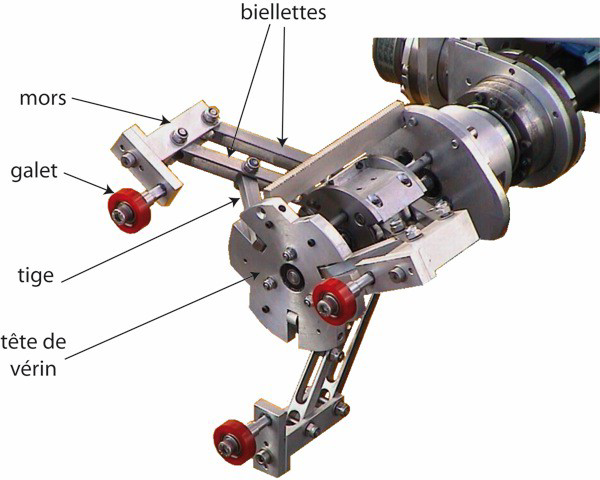
\includegraphics[width=.45\linewidth]{fig_23a.png}
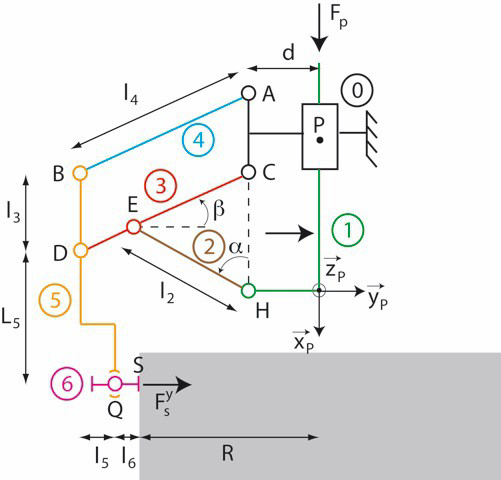
\includegraphics[width=.45\linewidth]{fig_23b.png}
\caption{Pince utilisée sur le système ROBOVOLC et schéma cinématique associé \label{fig_23}}
\end{figure} 
\fi 

\ifprof
\else

\noindent\footnotesize
 \fbox{\parbox{.9\linewidth}{
 Éléments de corrigé : 
 \begin{enumerate}
\item $h=1$.
%\item $h=8$.
%\item .
 \end{enumerate}}}
\normalsize

\begin{flushright}
\footnotesize{Corrigé  voir \ref{B2:16:71}.}
\end{flushright}%
\fi